% For Monday: 
% - explain why pointers are important
%  - this is the difference between good programmers and mediocre
%    programmers
%  - I have four objectives
%    * read code
%    - write code
%    * self-learn
%    
% Plus an exercise of "human pointers" to implement a Stack

\section{Interfaces}
\label{sec:interfaces}

Classes in Java have member fields and member methods. The fields are
variables stored inside objects for that class, and contain
information about the object. For example, they can represent the age
of a person or the number of patients in a hospital. The set of all
member fields of an object is usually called the \emph{state} of the
object: they say how the object \emph{is} at the current moment. 

On the other hand, methods (at least public ones) say what the object
can do. For example, a person can say something or a hospital can take
a new patient. The set of (public) methods of a class is usually
called the \emph{behaviour} of the class. 

The behaviour of a class is more important for a programmer than its
state. The state is an implementation detail that can change without
affecting its behaviour, and is usually not important for the task at
hand: this is why fields should be \verb+private+ in most
situations. If I want an object of type \verb+Person+ to say
something, I do not really mind if the person internally uses some
object of type \verb+VocalCord+, or some \verb+Vocoder+, or something
else: I just want the method to do what it is supposed to do. I do not
mind either if a future version of \verb+Person.say(String)+ is
implemented internally in a different way or with different
fields. Actually, it is quite common that the implementation changes
over time (to make it faster, or to use less memory, or to fix bugs)
so I should not worry about it; I should assume it will happen sooner
or later. 

This is why the behaviour of a class is more important than its
state. There are two consequences of this. First, the state should
always be private. Second, the behaviour must be easy to know and
understand without the need to read the whole code of my class. This
where interfaces come in. 

An interface in Java is just a way of showing and explaining the
behaviour of your class. An interface does not contain any information
at all about the implementation or the state of your class. It only
describes some (sometimes all) of the public methods of your
class. Let's see an example: 

\VerbatimInput[frame=single,label=Example]{src/Person.java}

As you can see, the definition of an interface is very similar to the
definition of a class, it is even defined in a java file. 
The difference (and it is a big one!) is that
there are no implementation details at all in the definition of the
interface. It only declares the methods: their names, and their
parameters. Every other detail about the class is left for the class
to be defined. 

There are two more things you may have noticed: 

\begin{itemize}
\item There is no need to say that methods are \verb+public+
  because methods defined on an interface are public by definition.
\item We have introduce new kind of comments, that start with
  \verb+/**+ and end with \verb+*/+ and can span several lines. These
  are called \emph{long comments} and are useful to document your
  code, especially methods, interfaces, and classes. The comments we
  already knew about, that start with \verb+//+ and go to the end of
  the line ---but not to the next line--- are called \emph{short
    comments}. 
\end{itemize}

A class that implements all the methods defined on an interface can
use the reserved keyword \verb+implements+ to mark it. This will tell
the Java compiler that the class must have the method on the
interface; if it does not, the compiler will complain with an error:
\verb+class is+ \verb+not abstract and+ \verb+does not override+
\verb+abstract method...+ 

Let's see three examples of classes that implement \verb+Person+:

\VerbatimInput[frame=single,label=Example]{src/AdultPerson.java}

\VerbatimInput[frame=single,label=Example]{src/KidPerson.java}

As you can see, both \verb+AdultPerson+ and \verb+KidPerson+ implement
the interface \verb+Person+, but they do it in different ways: 

\begin{itemize}
\item \verb+AdultPerson+ uses a member field called \verb+situation+
  while \verb+KidPerson+ uses a member field called
  \verb+position+. This is usually a sign that both classes have been
  coded by different programmers.
\item \verb+KidPerson+ only prints part of the message when told to
  say it.
\item \verb+KidPerson+ moves slower than \verb+AdultPerson+. The
  latter can move at two different speeds (\verb+run+ and
  \verb+walk+), one of them using more 
  energy than the other. \verb+KidPerson+ has unlimited energy. 
\end{itemize}

From the point of view of a programmer that want to use an object of
type \verb+Person+, all these differences may be irrelevant and
confusing. The programmer just wants an object that moves and says
things. This is possible thanks to interfaces. Look at the following
code: 

\begin{verbatim}
    Person son = new AdultPerson();
    // move in front of mother
    son.move(10);
    // give the message
    son.say("I love you, Mum.");
\end{verbatim}

This code will work exactly the same regardless of the specific class
that is used as long as it
implements the interface \verb+Person+. 

\subsection*{Exercise}
\label{sec:exercise}

Implement a simple class that executes the former code in its main
method. Change the class \verb+AdultPerson+ for \verb+KidPerson+ and
verify that it still compiles and runs. 

\section{Interfaces and data structures}
\label{sec:interfaces-lists}

Interfaces are very important in Java and in any modern
object-oriented programming language. Interfaces allow programmers to
\emph{hide the implementation} of their classes and expose only their
behaviours. This is good because other programmers can use their
classes with minimal effort: they only need to understand the
behaviours, not the full code. Using other programmers' classes (or
your own between different projects) is called \emph{code reuse}, and
saves a lot of effort to programmers (and money to their
companies). For example, you do not need to 
create a new \verb+String+ class every
time you want to write text in your programs: you just use the
\verb+String+ that comes with Java. And you do not need to understand
the code of the class\footnote{The code of all classes in the basic
  Java library is public. You can find it online. Java is free
  software under the GPL license.}, you only need to understand its
behaviour: what \verb+chatAt(int)+ does, what
\verb+substring(int,int)+ does, etc. This makes your life much easier
and is good. 

We have seen how dynamic data structures make it possible to store
unlimited amounts of data in a program (unlike arrays or discrete
variables). Now we are going to see three more special examples of
dynamic lists, and we will define them bu using interfaces. 

\subsection{Stacks}
\label{sec:stacks}

We are all familiar with the concept of stacks. When we are putting
books on a box, we usually pile them in stacks: one on top of the
next one, so we can only see the last one we have put it, i.e.~the one
on top. When we pile papers on a table we also create a stack. 

Stacks are very important in computing, and are used in many different
contexts. The method call stack that stores the variables for each
method in a program is just one well-known example. Every time you
call a method, you create a new level on the stack to store your
variables; while you are in the method, you can only ``see'' the
variables on your level; when you end the method, those variables are
forgotten and you see the variables on the former level (see
Figure~\ref{fig:stackparameter}).  

\begin{figure}[hbtp]
  \centering
  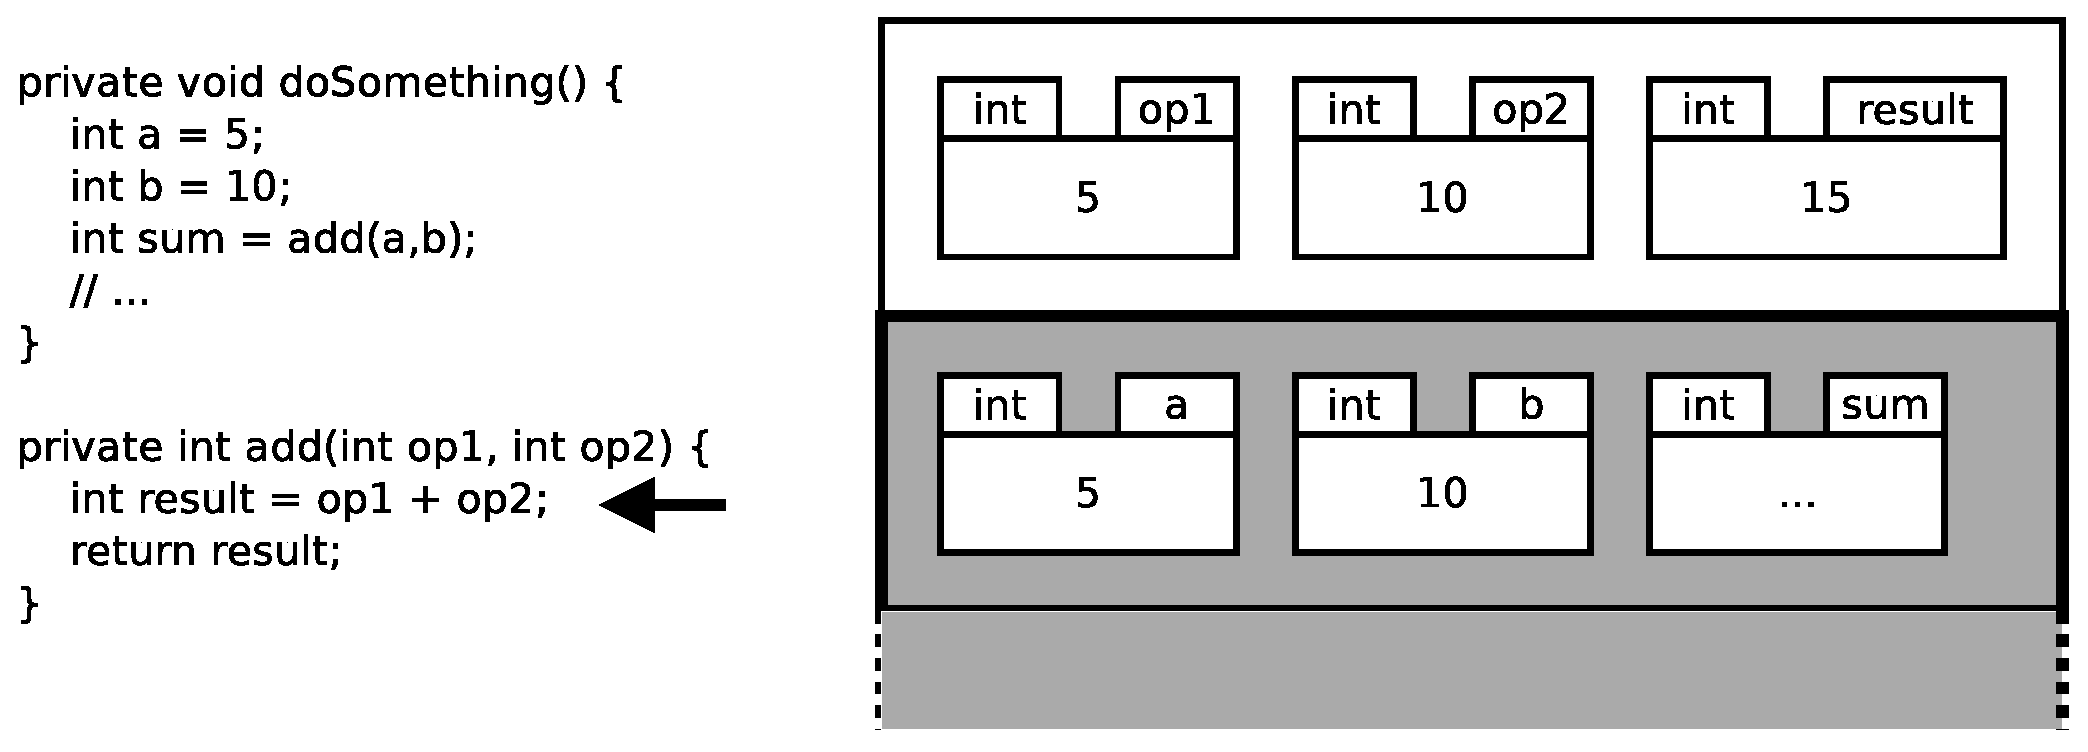
\includegraphics[width=\textwidth]{gfx/parameter-stack}
  \caption{The parameter stack is an example of a stack
    structure. When method is called (add), a new level is put on the
    stack to store the parameters and the local variables. While in
    the method, the variables of the other method (a, b, sum) cannot
    be accessed: they are on a different level of the stack, and only
    the most recent one is accessible.}
  \label{fig:stackparameter}
\end{figure}

In a stack, only the last level is accessible: all former levels are
hidden until the last level is removed. This is why stacks are called
LIFO structures: Last In, First Out. A Stack is defined by the
following methods:  

\begin{description}
\item[push(...)] inserts an element at the beginning of the stack.
\item[pop(...) ] remove an element from the \emph{beginning} of the stack.
\item[empty(...) ] returns true if there are no elements on the stack,
  false otherwise.
\end{description}



%              interfaces
%              queues and stacks, 
%              trees, binary and non-binary trees, 
%              basics of memory allocation, gargage collection, 


%%% Local Variables:
%%% mode: latex
%%% TeX-master: "main"
%%% End:
